\documentclass[twoside]{article}

\usepackage[sc]{mathpazo}
\usepackage[T1]{fontenc}
\usepackage{microtype}
\usepackage{color}
\usepackage[twoside,height=24cm,left=3cm]{geometry}
\usepackage{multicol}
\usepackage[hang, small,labelfont=bf,up,textfont=it,up]{caption}
\usepackage{booktabs}
\usepackage{float}
\usepackage{hyperref}
\usepackage[spanish]{babel}
\usepackage[utf8]{inputenc}
\usepackage{graphicx}
\usepackage{amsmath}
\usepackage{amssymb}
\usepackage{enumerate}
\usepackage{bm}
\usepackage{lettrine}
\usepackage{paralist}
\usepackage{abstract}
\usepackage{titlesec}
\usepackage{fancyhdr}
\usepackage{fullpage}
\usepackage{booktabs}
\usepackage{tikz}
\usepackage{pgfplots}
\usepackage{float}
\usepackage{hyperref}
\usepackage{color}
\usepackage{graphicx}
\usepackage{xfrac}
\usepackage{titling}
\usepackage{multirow}
\usepackage{subcaption}
\usepackage{natbib}
\usepackage{siunitx}
\usepackage[format=plain,labelfont=it,textfont=it]{caption}
\usepackage{geometry}
\usepackage{multicol}

\renewcommand{\abstractnamefont}{\normalfont\bfseries}
\renewcommand{\abstracttextfont}{\normalfont\small\itshape}
\newcommand{\grad}{$^{\circ}$}

\linespread{1.05}
\setlength\parindent{0pt}
\setlength\columnsep{20pt}
\setlength{\headheight}{12.0pt}
\addto\captionsspanish{
    \def\contentsname{\'Indice}
    \def\bibname{Referencias}
    \def\tablename{Tabla}
    \def\abstractname{Resumen}
}
\pagestyle{fancy}
\fancyhead{}
\fancyfoot{}
\fancyhead[C]{Laboratorio 7 $\bullet$ Cátedra Ledesma}
\fancyfoot[RO,LE]{\thepage}
\hyphenpenalty=100000
\pgfplotsset{compat=1.10}
\geometry{left=15mm,right=15mm}

\begin{document}

\begin{titlepage}
\begin{center}

\textsc{\LARGE Laboratorio 7}\\[0.5cm]
\textsc{\Large Departamento de Física}\\[0.5cm]
\textsc{\Large Facultad de Ciencias Exactas y Naturales}\\[0.5cm]
\textsc{\Large Universidad de Buenos Aires}\\[1.5cm]

1er cuatrimestre 2021\\[1.5cm]

{ \huge \bfseries Aplicación del efecto Josephson a la generación de señales arbitrarias con aplicaciones a la metrología}\\[1.5cm]


%\begin{minipage}{0.8\textwidth}
%\begin{flushleft} \large


Alumno:
Pinto Zárate, José Daniel\\
\href{mailto:dann.2207@gmail.com}{dann.2207@gmail.com}

%\end{flushleft}
%\end{minipage}
\vfill
{\large \today}
\end{center}
\end{titlepage}

\begin{abstract}

    En este trabajo se armó e implementó un sistema Josephson pulsado (JAWS)

\end{abstract}

\begin{multicols}{2}

\section{Introducción}

El efecto Josephson es un fenómeno que se presenta en las junturas superconductoras, como la que se muestra en la figura \ref{fig:intro_junturaJosephson}, cuando a estas se las somete a diferentes señales de corriente en la frecuencia de las microonda. Hay varios tipos de este efecto, y en particular en este trabajo se considera el efecto Jospephson pulsado, que es cuando se envía un tren de pulsos de microondas a un array de junturas Josephson en serie. Otros efectos relacionados son el efecto Josephson AC, que es cuando . Dichos efectos estan entre los que se utilizan para construir otros sintetizadores que aprovechan el mismo fenómeno, como el sistema Josephson programable (PJVS), o el convencional (CJVS). 

El efecto josephson pulsado consiste en una conversión entre una señal de tren de pulsos AC,  y 



\begin{figure}[H]
    \centering
    \includegraphics[width=\linewidth]{figuras/intro/junturaJosephson.png}
    \caption{Efecto Josephson en una juntura superconductora}
    \label{fig:intro_junturaJosephson}
\end{figure}



Un plateau es una zona de la curva I-V en la que la tensión es constante en un rango contínuo de corrientes. Si la corriente que atraviesa el JAWS se mantiene dentro de una de estas zonas, se verifica la ecuación de Josephson.
La corriente de compensación se agrega para que el array se encuentre en un plateau, como se muestra en la figura \ref{fig:intro_plateau}. La señal debe estar en un plateau ya que es un requisito para que se verifique la ecuaciónde Josephson.

Si el sistema se encuentra en un plateau, se cuantiza el área de la curva de corriente vs tiempo, de modo que aunque los pulsos se deformen, siempre que mantengan su área, se obtendrán los mismos resultados \cite{benz1998}.

El cambio de temperatura es un factor que puede alterar la forma de estos pulsos, y una posible fuente de error. Si por ejemplo los pulsos se ensanchan hasta unirse, se podría perder información de la señal en las zonas en las que haya alta densidad de pulsos.

\begin{figure}[H]
    \centering
    \includegraphics[width=\linewidth]{figuras/intro/plateau.png}
    \caption{Señal corrida a la derecha del plateau}
    \label{fig:intro_plateau}
\end{figure}

\section{Descripción de la simulación numérica}

El código utilizado genera distintas variables presentes en la modulación sigma delta, y permite hacer un análisis muy detallado a partir de las mismas. En la figura \ref{fig:bloques} se muestra el diagrama de bloques representativo del algoritmo de modulación de 1er orden \cite{script}.

\begin{figure}[H]
\centering
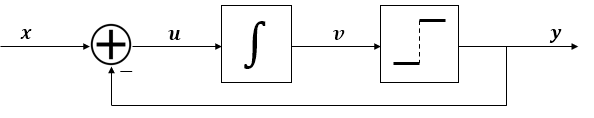
\includegraphics[width=\linewidth]{figuras/bloques_1erorden.png}
\caption{Diagrama de bloques correspondiente a la modulación $\Sigma\Delta$ de 1er orden}
\label{fig:bloques}
\end{figure}

En el apéndice se describe muy brevemente como se leen estos diagramas, y como se pueden traducir a un método iterativo en las 4 variables presentes: $x,u,v,y$.
La primera, $x$, representa la señal analógica de entrada, que es la señal que queremos generar. $u$ y $v$ son variables auxiliares, en donde $v$ es la integral de $u$, y $u$ es la diferencia $x-y$. $y$ es la salida final del cuantizador, que tiene en nuestro caso solo 2 valores posibles.


En este trabajo se implementó, siguiendo diferentes publicaciones (\cite{delarosa2011}, \cite{aziz1996}), el algoritmo de modulación Sigma-Delta de 1er orden en Python. Esto permitió explorar diferentes aspectos del método que no eran muy accesibles desde otras implementaciones, de manera muy sencilla.
Las implementaciones anteriores contienen optimizaciones adicionales que por el momento nuestro código no incluye. La más conocida es el paquete de Matlab de Richard Scherier \cite{DSmatlab}, sobre la cual se basa el paquete de Python de G. Venturini \cite{DSpython}. %Este último paquete fue usado para contrastar cualitativamente los pulsos generados por nuestro código, además de los resultados obtenidos en simulaciones numéricas de distintas fuentes \cite{aziz1996}, \cite{delarosa2011}.

En la figura \ref{fig:integrador} se muestra mejor el comportamiento de las variables $u$ y $v$ para cuando se quiere generar una señal DC de valor 0.8 u.a. Se observa que hay un período en el que la señal $u=x-y$ es ligeramente negativa, esto es porque $x=0.8$ es ligeramente inferior al nivel superior $y=1$ (todo en unidades arbitrarias). Durante este período, se van sumando estos valores de $u$ al valor de $v$, que en la figura \ref{fig:integrador} es la pendiente negativa que está en el área de integración negativa, sombreada en azul.


\begin{figure}[H]
\centering
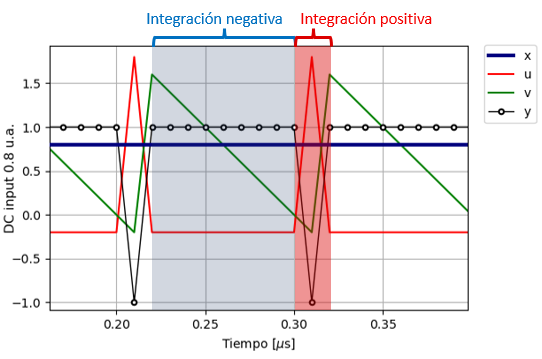
\includegraphics[width=\linewidth]{figuras/integracion.png}
\caption{Ejemplo del funcionamiento del integrador en la modulación a 1er orden}
\label{fig:integrador}
\end{figure}

Llega un punto en que $v$ pasa a ser negativo, de modo que, al pasar al cuantizador, generará un pulso $y$ negativo, luego de varios positivos. Esto es lo que se ve en el área de integración positiva: el valor de $u$, en ese lapso muy corto de tiempo, es positivo y muy grande, de tal manera que basta solo uno para volver al régimen de pulsos positivos. De esta manera el algoritmo genera la proporción de pulsos negativos y positivos deseada.

\section{Descripción del experimento}

El esquema experimental del JAWS se muestra en la figura \ref{fig:experimental_1}. Se utilizó un generador de pulsos programable (FPGA) Xilinx Zynq-7000, que enviaba pulsos de corriente a una frecuencia de \SI{5}{\giga\hertz}. Dicho FPGA tiene tres patrones de calibración, que se usaran para calibrar los pulsos programados. Estos pulsos son enviados mediante un cable semirrígido, que soporta el rango de frecuencias utilizado en el experimento, y viajan hacia el array sumergido en Helio líquido a \SI{4.2}{\kelvin}

\begin{figure}[H]
    \centering
    \includegraphics[width=0.75\linewidth]{figuras/experimental/1.png}
    \caption{Esquema del arreglo experimental para la prueba del JAWS}
    \label{fig:experimental_1}
\end{figure}

A la señal de pulsos de la FPGA se le agrega una corriente adicional de frecuencia \SI{3.125}{\kilo\hertz} mediante un generador de funciones (Tektronix AFG1062), dicha señal es la corriente de compensación.

En la figura XXX se muestra un detalle de como se suman las señales de pulsos con la corriente de compensación. El chip JAWS tiene pines por los que entra dicha corriente, mientras que los pulsos entran a través de la entrada externa, mediante el cable semirrígido.

\section{Resultados y Análisis}

    \subsection{Simulación numérica}

    Usando nuestro script \cite{script}, generamos los pulsos correspondientes a una señal DC para reproducir los resultados que se muestran en \cite{aziz1996}. En la figura 

    \subsection{Pruebas experimentales con la FPGA}

    En la figura \ref{fig:resultados_patron32FPGA} se muestran las mediciones de la calibración de la FPGA. Se puede ver como se deforman los pulsos de corriente.

    \begin{figure}[H]
        \centering
        \includegraphics[width=0.75\linewidth]{figuras/resultados/patron32FPGA.png}
        \caption{Medición de la salida de la FPGA en el modo de patrón de 1 pulso cada 32}
        \label{fig:resultados_patron32FPGA}
    \end{figure}



\end{multicols}

%\newpage
\bibliographystyle{unsrt}
\bibliography{references.bib}


\nocite{*} % Insert publications even if they are not cited in the poster

\end{document}
